%%%%%%%%%%%%%%%%%%%%%%%%%%%%%%%%%%%%%%%%%
% Short Sectioned Assignment LaTeX Template Version 1.0 (5/5/12)
% This template has been downloaded from: http://www.LaTeXTemplates.com
% Original author:  Frits Wenneker (http://www.howtotex.com)
% License: CC BY-NC-SA 3.0 (http://creativecommons.org/licenses/by-nc-sa/3.0/)
%%%%%%%%%%%%%%%%%%%%%%%%%%%%%%%%%%%%%%%%%

%----------------------------------------------------------------------------------------
%	PACKAGES AND OTHER DOCUMENT CONFIGURATIONS
%----------------------------------------------------------------------------------------

\documentclass[paper=a4, fontsize=11pt]{scrartcl} % A4 paper and 11pt font size

% ---- Entrada y salida de texto -----

\usepackage[T1]{fontenc} % Use 8-bit encoding that has 256 glyphs
\usepackage[utf8]{inputenc}
%\usepackage{fourier} % Use the Adobe Utopia font for the document - comment this line to return to the LaTeX default


\usepackage[utf8]{inputenc}
\usepackage[T1]{fontenc}
\usepackage[spanish]{babel}
\usepackage{times}

\usepackage{color}
\definecolor{gray97}{gray}{.97}
\definecolor{gray75}{gray}{.75}
\definecolor{gray45}{gray}{.45}

\usepackage{listings}
\lstset{ frame=Ltb,
	framerule=0pt,
	aboveskip=0.5cm,
	framextopmargin=3pt,
	framexbottommargin=3pt,
	framexleftmargin=0.4cm,
	framesep=0pt,
	rulesep=.4pt,
	backgroundcolor=\color{gray97},
	rulesepcolor=\color{black},
	%
	stringstyle=\ttfamily,
	showstringspaces = false,
	basicstyle=\small\ttfamily,
	commentstyle=\color{gray45},
	keywordstyle=\bfseries,
	%
	numbers=left,
	numbersep=15pt,
	numberstyle=\tiny,
	numberfirstline = false,
	breaklines=true,
}

% minimizar fragmentado de listados
\lstnewenvironment{listing}[1][]
{\lstset{#1}\pagebreak[0]}{\pagebreak[0]}

\lstdefinestyle{consola}
{basicstyle=\scriptsize\bf\ttfamily,
	backgroundcolor=\color{gray75},
}

\lstdefinestyle{C}
{language=C,
}
% ---- Idioma --------

\usepackage[spanish, es-tabla]{babel} % Selecciona el español para palabras introducidas automáticamente, p.ej. "septiembre" en la fecha y especifica que se use la palabra Tabla en vez de Cuadro
% ---- Otros paquetes ----

\usepackage{amsmath,amsfonts,amsthm} % Math packages
%\usepackage{graphics,graphicx, floatrow} %para incluir imágenes y notas en las imágenes
\usepackage{graphics,graphicx, float} %para incluir imágenes y colocarlas

% Para hacer tablas comlejas
%\usepackage{multirow}
%\usepackage{threeparttable}

%\usepackage{sectsty} % Allows customizing section commands
%\allsectionsfont{\centering \normalfont\scshape} % Make all sections centered, the default font and small caps

\usepackage{fancyhdr} % Custom headers and footers
\pagestyle{fancyplain} % Makes all pages in the document conform to the custom headers and footers
\fancyhead{} % No page header - if you want one, create it in the same way as the footers below
\fancyfoot[L]{} % Empty left footer
\fancyfoot[C]{} % Empty center footer
\fancyfoot[R]{\thepage} % Page numbering for right footer
\renewcommand{\headrulewidth}{0pt} % Remove header underlines
\renewcommand{\footrulewidth}{0pt} % Remove footer underlines
\setlength{\headheight}{13.6pt} % Customize the height of the header

\numberwithin{equation}{section} % Number equations within sections (i.e. 1.1, 1.2, 2.1, 2.2 instead of 1, 2, 3, 4)
\numberwithin{figure}{section} % Number figures within sections (i.e. 1.1, 1.2, 2.1, 2.2 instead of 1, 2, 3, 4)
\numberwithin{table}{section} % Number tables within sections (i.e. 1.1, 1.2, 2.1, 2.2 instead of 1, 2, 3, 4)

\setlength\parindent{0pt} % Removes all indentation from paragraphs - comment this line for an assignment with lots of text

\newcommand{\horrule}[1]{\rule{\linewidth}{#1}} % Create horizontal rule command with 1 argument of height


\begin{document}
\title{
\normalfont \normalsize 
\textsc{{\bf Metaheurísticas (2015-16) \\ Grado en Ingeniería Informática \\ Universidad de Granada} \\ [25pt] % Your university, school and/or department name(s)
\horrule{0.5pt} \\[0.4cm] % Thin top horizontal rule
\huge Práctica 5: Búsquedas con técnicas híbridas. \\ % The assignment title
\horrule{2pt} \\[0.5cm] % Thick bottom horizontal rule
}}
\author{Miguel López Campos\\ 54120359W\\ miguelberja@correo.ugr.es\\ Grupo Viernes 18:30} % Nombre y apellidos


\date{\normalsize\today} % Incluye la fecha actual
%----------------------------------------------------------------------------------------
% DOCUMENTO
%----------------------------------------------------------------------------------------


	
	\maketitle % Muestra el Título
	\newpage %inserta un salto de página
	
	\tableofcontents % para generar el índice de contenidos
	\listoffigures

	
	\newpage
	
	\
	
	
	
	\section{Descripción del problema}
	El problema que estamos abordando es la selección de características. Este problema es muy útil en el campo de "machine learning".
	\\
	\\
	Tenemos un conjunto de datos de entrenamiento y otro de validación, ambos etiquetados o clasificados. Lo que queremos hacer es 'aprender' una función que a partir de las características del conjunto de datos de entrenamiento, nos permita estimar el etiquetado de otros vectores de características. Lo que nosotros queremos hacer es eliminar las características que no son relevantes en el problema, eliminando de esta manera ruido en el conjunto de datos y mejorando la eficiencia de nuestro clasificador. Es decir, no sólo mejoraremos el tiempo, si no muy probablemente la calidad de nuestras soluciones también (en cuanto al error se refiere).
	\\
	\\
	La gran dificultad de este problema radica en el gran número de soluciones posibles, llevándonos al punto de que un algoritmo Greedy que nos garantice la solución óptima podría llevarnos días de ejecución para determinados problemas. Es por esto por lo que tenemos que usar Metaheurísticas. Necesitamos soluciones buenas (aunque no sea la mejor) en un tiempo menor.
	\\
	\\
	Nosotros usaremos para clasificar el algoritmo 3NN. Lo que hace este algoritmo es calcular la distancia euclídea entre el vector de características al cual queremos estimar una clase y el resto de vectores de características del conjunto de entrenamiento. Lo que hace el 3NN es coger los 3 elementos menos distantes y la clase mayoritaria entre esos 3 será la estimación que haremos.
	\\
	\\
	Validaremos con la técnica 5x2 Cross Validation. Usaremos 5 particiones de los datos distintas al 50\% (y aleatorias) y aprenderemos el clasificador con una submuestra y validaremos con la otra y después al contrario. Con esta técnica tendremos el porcentaje de acierto, que nos servirá para ver la calidad de nuestro algoritmo.
	\\
	\\
	Otros datos con los que valoraremos la calidad de nuestros algoritmos serán los tiempos de ejeución y los porcentajes de reducción, es decir, el porcentaje de características que hemos reducido.
	\\
	\\
	Con nuestras metaheurísticas querremos optimizar la función de acierto. Es decir, queremos maximizar el acierto, siendo la función:\\
	$tasaclass = 100*\frac{nºinstancias bien clasificadas}{nº instancias Total}$
	
	\newpage
	
	
	\section{Descripción de los aspectos comunes de los algoritmos}
	La práctica ha sido desarrollada en C++.
	\\
	
	\begin{enumerate}
		\item Representación de las soluciones. Para representar las soluciones utilizaremos un array de booleanos. Será común a todos los algoritmos. Si la componente $i$ es true, esto indicará que la característica $i$ se tendrá en cuenta (no ha sido eliminada).
		
		\item Función objetivo. La función que queremos optimizar se trata del porcentaje de acierto de estimaciones de clases, descrita en el apartado anterior.
		\\
		\\
		En pseudocódigo es la siguiente:
		\begin{lstlisting}
funcion_objetivo(conjunto_training, caracteristicas_activas)
begin
  Para todo elemento i del conjunto_test
  begin
    elemento <- elemento i del conjunto_training
	clase <- 3NN(conjunto_training-{elemento}, elemento, caracteristicas_activas)
				
	Si la clase estimada por 3NN se corresponde a la clase real -> aciertos++
  end
			
  promedio <- aciertos/tamaño conjunto_test
			
  devolver promedio
end
		\end{lstlisting}
		
		\item Función clasificadora. Como función clasificadora usaremos el algoritmo 3NN, descrito anteriormente.
		\\
		\\
		\newpage
		
		El pseudocódigo es el siguiente:
		\begin{lstlisting}
3NN(conjunto_training, vector_caracteristicas, caracteristicas_activas)
begin
  Para cada vector i de caracteristicas de training
  begin
  
    array_distancias.añadir(distanciaeuclidea(i, vector_caracteristicas, caracteristicas_activas))
    
   end
   
  minimo1 <- minimo(array_distancias)
  minimo2 <- minimo(array_distancias-minimo1)
  minimo3 <- minimo(array_distancias-minimo1-minimo2)
  
  Si la clase de vector_caracteristicas[minimo2]==clase de vector_caracteristicas[minimo3] entonces
    La clase del vector de caracteristicas es esa
  Si no
    La clase del vector de caracteristicas es la clase de vector_caracteristicas[minimo1]
    
  devolver clase del vector de caracteristicas
  
end
		\end{lstlisting}
		
		\item Función para la generación de soluciones aleatorias
\begin{lstlisting}
PRE: solucion está inicialmente entero a falso

Generar_solucion_aleatoria(solucion, tamanio_solucion)
begin
  indices_disponibles <- [0...tamanio_solucion-1]
  caracteristicas_a_cambiar <- Random(0, tamanio_solucion-1)
  
  Para i=0 hasta caracteristicas_a_cambiar
  begin
    caracteristica <- Random(0, indices_disponibles.length-1)
    solucion[indices_disponibles[caracteristica]] <- true
    indices_disponibles-{caracteristica}    //Elimino el indice de la caracteristica para no volver a cambiarla
  end
  
  devolver solucion
end

\end{lstlisting}
		
		\item Antes de trabajar con cualquier algoritmo hay que normalizar los conjuntos de datos.
		
		\item El criterio de parada para los algoritmos genéticos es que realicen 15000 evaluaciones de la función objetivo.
		
		\item Para cada algoritmo he plantado el mismo valor de semilla para una correspondiente iteración.
		
		\item He usado para tomar tiempos y para crear números aleatorios las funciones dadas en decsai.
	\end{enumerate}
	
	\section{Algoritmo de comparación SFS}
	El algoritmo de comparación SFS es muy simple. Primero se genera una solución con todo a
	falso. A partir de aquí, exploramos todo el vector solución y cogemos la característica con la que
	vayamos a obtener mayor ganancia. Una vez la escojamos, volvemos a realizar otra iteración cogiendo la siguiente característica que nos de más ganancia y así sucesivamente. El algoritmo acaba cuando ya no haya mejora en una búsqueda completa sobre el vector solución.
	\\
	\\
	La descripción en pseudocódigo del algoritmo es la siguiente:
	\begin{lstlisting}
SFS(training, Solucion, Tasa_Solucion)
begin
  mejor_solucion <- 0.0
  mejora <- true
  
  Mientras mejora
  begin
    mejora <- false
    S_tmp <- Solucion
    
    Para i=0 hasta S_tmp.length
    begin
      Si S_tmp[i] es false entonces
        S_tmp[i] <- true
        S_tmp_tasa <- funcion_objetivo(training, S_tmp)
        
        Si S_tmp_tasa es mejor que mejor_solucion entonces
          mejor_solucion <- S_tmp_tasa
          mejora <- true
          Solucion <- S_tmp
          
        S_tmp[i] <- false
    end
  end
  
  devolver Solucion y mejor_solucion //Por referencia
  
end
	\end{lstlisting}


	\section{Algoritmo genético generacional}
	En los algoritmos genéticos generacionales, en cada nueva iteración, se reemplaza toda la población por la nueva.
	Los parámetros usados son 0.7 para la probabilidad de cruce y 0.001 para la probabilidad de mutación. Ambas probabilidades son las dadas por el guión de la práctica. Como criterio de parada he puesto que se realicen un máximo de 15000 evaluaciones de la función objetivo. Para mantener el elitismo, me aseguro de que la mejor solución de una población anterior se encuentra en la nueva población cambiándola por la peor de esta última (en el caso de que sea mejor).
	\\
	\\
	El mecanismo de selección que he empleado consiste en realizar tantos concursos binarios aleatorios como cromosomas hay en la población (en nuestro caso 30). Los ganadores de estos concursos binarios serán los cromosomas de nuestra población seleccionada. La descripción en pseudocódigo es la siguiente:
	
	\begin{lstlisting}
seleccionar(poblacion, tasas_poblacion, seleccion, tasas) //Por referencia 
begin
  seleccion <- Array() //Array de cromosomas (vectores solucion)
  tasas <- Array() //Tasas de los seleccionados
  
  disponibles <- 0..poblacion.length-1 //Array de índices para controlar que no compite un cromosoma consigo mismo
  
  Para i=0 hasta poblacion.length
  begin
    aux <- disponibles
    
    random1 <- Random(0, aux.length-1) //Random devuelve un entero
    aux <- aux-{random1} //Me aseguro de que no cojo el mismo cromosoma
    random2 <- Random(0, aux.length-1)
    
    aux <- disponibles
    
    Si tasas_poblacion[random1] es mejor que tasas_poblacion[random2] entonces
      seleccion.aniadir(poblacion[random1])
      tasas.aniadir(tasas_poblacion[random1])
    si no entonces
      seleccion.aniadir(poblacion[random2])
      tasas.aniadir(tasas_poblacion[random2])
    
  end
  
  devolver seleccion y tasas //Por referencia
  
end
	\end{lstlisting}
	
Para la fase de cruce lo que hago es de la selección obtenida de la fase de selección, cruzo el primero con el segundo, el segundo con el tercero, etc. hasta cubrir el número esperado de cruces, calculado con la fórmula $ProbabilidadCruce * (NumeroCromosomas/2)$. Lo que hago es elegir dos puntos de corte (asegurándome de que no son el mismo porque si no no cruzarían nada) y los elementos del cromosoma (o vector solución) que están entre esos dos puntos de corte son los que se intercambiarán un padre y otro, es decir, los nuevos cromosomas serán ellos mismos pero cada uno con la parte de central del otro. Estos puntos de corte además tienen que ir desde la segunda componente del array hasta la penúltima. La función de cruce es la siguiente:
\begin{lstlisting}
cruce(padre1, padre2) //por referencia
begin
  posibles <- 0..padre1.length-1 //Numero de caracteristicas del vector solucion
  
  corte1 <- posibles[Random(1, posibles.length-2)]
  posibles <- posibles-{corte1}
  corte2 <- posibles[Random(1, posibles.length-2)]
  
  Si corte1 > corte2 entonces
    hago swap entre corte1 y corte2
    
  aux1 <- padre1[corte1..corte2] //Cojo la parte central del array
  aux2 <- padre2[corte1..corte2]
  
  padre1 <- padre1-padre1[corte1..corte2] //Elimino la parte central del array
  padre2 <- padre2-padre2[corte1..corte2]
  
  padre1.insertar(aux2, corte1) //Inserto la parte central del otro padre a partir de cote1
  padre2.insertar(aux1, corte1)
  
  
  devolver padre1 y padre2 //por referencia
  
end
\end{lstlisting}


Para la mutación, al igual que con los cruces, calculo el número esperado de mutaciones que se van a realizar. Para ello uso la fórmula $ProbabilidadMutacion * numeroCromosomas * numeroGenes$. Siendo la probabilidad de mutación 0.001. La función con la que muto es la siguiente:

\begin{lstlisting}
mutar(solucion, i) //Muto la componente i de solucion
begin
  Si solucion[i] es true entonces lo pongo a false
  si no lo pongo a true
  
  devolver solucion
  
end
\end{lstlisting}

El algoritmo completo en pseudocódigo es el siguiente:
\begin{lstlisting}
//PRE: Solucion inicialmente es entero falso

AGG(training, Solucion, Tasa_Solucion)
begin
  poblacion <- Array() //Array de vectores solucion
  tasas_poblacion <- Array() //Array de las tasas de la poblacion
  
  Para i=0 hasta 30
  begin
    tmp <- generar_solucion_aleatoria(Solucion, Solucion.length)
    poblacion.aniadir(tmp)
    tasa <- funcion_objetivo(training, tmp)
    tasas_poblacion.aniadir(tasa)
  end
  
  
  Para i=0 hasta 15000
  begin
    //Guardo el mejor elemento de la poblacion
    indice_mejor <- maximo(tasas_poblacion)
    mejor <- poblacion[indice_mejor]
    
    Seleccion <- Array() //Array de vectores solucion
    Tasas_Seleccion <- Array() //Array de tasas
    
    
    //Fase de seleccion
    seleccionar(poblacion, tasas_polacion, Seleccion, Tasas_Seleccion) //Por referencia
    
    //Fase de cruce
    n_cruces <- 0.7*30/2
    
    Para j=0 hasta n_cruces
    begin
      padre1 <- Seleccion[2*j]
      padre2 <- Seleccion[2*j+1]
      
      cruce(padre1, padre2)
    end
    
    //Fase de mutación
    n_mutaciones <- 0.001*30*Seleccion[1].length
    
    Para j=0 hasta n_mutaciones
    begin
      r1 <- Random(0, Seleccion.length-1)
      r2 <- Random(0, Seleccion[r1].length-1)
      
      mutar(Seleccion[r1], r2)
    end
    
    
    //Fase de reemplazamiento
    Para j=0 hasta 30
    begin
      tasas_Seleccion[j] <- funcion_objetivo(training, seleccion[j])
    end
    
    encontrado <- Buscar(mejor) //Busco si está la mejor solucion anteriormente guardada
    
    Si !encontrado entonces
      min <- minimo(tasas_seleccion)
      
      Si tasas_seleccion[min] < tasas_poblacion[ind_mejor] entonces
        seleccion[min] <- mejor
        tasas_seleccion[min] <- tasas_poblacion[ind_mejor]
        
    poblacion <- seleccion
    tasas_poblacion <- tasas_seleccion
  end
  
  ind_max <- maximo(tasas_poblacion)
  solucion <- poblacion[ind_max]
  Tasa_Solucion <- Tasas_poblacion[ind_max]
  
  devolver solucion y Tasa_Solucion //Por referencia
  
end
\end{lstlisting}
NOTA: El incremento de la i en el bucle más externo lo hago de 30 en 30 ya que en cada iteración se realizan 30 evaluaciones de la función objetivo.

\section{Algoritmo de búsqueda local}
En la práctica hemos hibridado el algoritmo genético generacional con búsqueda local (con una sola iteración). La búsqueda local en pseudocódigo (de una sola iteración) es la siguiente:

\begin{lstlisting}
busqueda_local(training, Solucion, Tasa_Solucion)
begin
  Tasa_Solucion <- funcion_objetivo(training, Solucion)

  S <- Solucion

  repetidos <- [0...S.length-1]
    
  Mientras que no se mejore y mientras que no se haya generado todo el entorno de S
  begin
    S <- flip(S, repetidos) //Con repetidos evitamos repetir dos 			//soluciones de un mismo entorno

    coste_S <- funcion_objetivo(training, test, S)

    Si coste_S es mejor que Toste_Solucion entonces
    //S mejora a Solucion
      Solucion <- S
      Tasa_Solucion <- coste_S

  end
  
  devolver Solucion y Toste_Solucion //Por referencia
  
end
\end{lstlisting}

La descripción del generador de vecinos flip es la siguiente:
\begin{lstlisting}
Flip(Solucion, Repetidos)
begin
  random <- Random(0, Repetidos.length-1)

  index <- Repetidos[random]

  Si Solucion[index] es true lo cambio a false
  si no lo cambio a true

  Repetidos-{random}


  devolver Solucion
end
\end{lstlisting}


\section{Algoritmo memético 1}
En este algoritmo memético aplicaremos una búsqueda local a toda la población cada 10 generaciones. Llevaremos un contador de generaciones. Cuando llegue a 10 haremos búsqueda local a todos los cromosomas de la población y reinicializaremos la cuenta de generaciones. La descripción en pseudocódigo es la siguiente:
\begin{lstlisting}
AM1(training, Solucion, Tasa_Solucion)
begin
  poblacion <- Array() //Array de vectores solucion
  tasas_poblacion <- Array() //Array de las tasas de la poblacion

  Para i=0 hasta 30
  begin
    tmp <- generar_solucion_aleatoria(Solucion, Solucion.length)
    poblacion.aniadir(tmp)
    tasa <- funcion_objetivo(training, tmp)
    tasas_poblacion.aniadir(tasa)
  end

  
  generacion <- 0 //contador de generaciones

  Mientras no se realicen mas de 15000 evaluaciones
  begin
  //Guardo el mejor elemento de la poblacion
    indice_mejor <- maximo(tasas_poblacion)
    mejor <- poblacion[indice_mejor]

    Seleccion <- Array() //Array de vectores solucion
    Tasas_Seleccion <- Array() //Array de tasas


    //Fase de seleccion
    seleccionar(poblacion, tasas_polacion, Seleccion, Tasas_Seleccion) //Por referencia

    //Fase de cruce
    n_cruces <- 0.7*30/2

    Para j=0 hasta n_cruces
    begin
      padre1 <- Seleccion[2*j]
      padre2 <- Seleccion[2*j+1]

      cruce(padre1, padre2)
    end

    //Fase de mutación
    n_mutaciones <- 0.001*30*Seleccion[1].length

    Para j=0 hasta n_mutaciones
    begin
      r1 <- Random(0, Seleccion.length-1)
      r2 <- Random(0, Seleccion[r1].length-1)

      mutar(Seleccion[r1], r2)
    end


    //Fase de reemplazamiento
    Para j=0 hasta 30
    begin
      tasas_Seleccion[j] <- funcion_objetivo(training, seleccion[j])
    end

    encontrado <- Buscar(mejor) //Busco si está la mejor solucion anteriormente guardada

    Si !encontrado entonces
      min <- minimo(tasas_seleccion)

      Si tasas_seleccion[min] < tasas_poblacion[ind_mejor] entonces
        seleccion[min] <- mejor
        tasas_seleccion[min] <- tasas_poblacion[ind_mejor]

    poblacion <- seleccion
    tasas_poblacion <- tasas_seleccion
    
    generacion <- generacion+1
    
    Si generacion==10 entonces
      Para cada soluion j de poblacion
      begin
        poblacion[j] <- busqueda_local(training, poblacion[j], tasas_poblacion[j]) //tasas_poblacion por referencia
        
      end
  end

  ind_max <- maximo(tasas_poblacion)
  solucion <- poblacion[ind_max]
  Tasa_Solucion <- Tasas_poblacion[ind_max]

devolver solucion y Tasa_Solucion //Por referencia

end
\end{lstlisting}

\section{Algoritmo memético 2}
En este algoritmo también hibridaremos búsqueda local y el algoritmo genético generacional. Ahora la mutación se realizará sobre los cromosomas con una probabilidad p=0.1.
\begin{lstlisting}
//PRE: Solucion inicialmente es entero falso

AM2(training, Solucion, Tasa_Solucion)
begin
  poblacion <- Array() //Array de vectores solucion
  tasas_poblacion <- Array() //Array de las tasas de la poblacion

  Para i=0 hasta 30
  begin
    tmp <- generar_solucion_aleatoria(Solucion, Solucion.length)
    poblacion.aniadir(tmp)
    tasa <- funcion_objetivo(training, tmp)
    tasas_poblacion.aniadir(tasa)
  end

  generacion <- 0

  Mientras no se realicen mas de 15000 evaluaciones
  begin
    //Guardo el mejor elemento de la poblacion
    indice_mejor <- maximo(tasas_poblacion)
    mejor <- poblacion[indice_mejor]

    Seleccion <- Array() //Array de vectores solucion
    Tasas_Seleccion <- Array() //Array de tasas


    //Fase de seleccion
    seleccionar(poblacion, tasas_polacion, Seleccion, Tasas_Seleccion) //Por referencia

    //Fase de cruce
    n_cruces <- 0.7*30/2

    Para j=0 hasta n_cruces
    begin
      padre1 <- Seleccion[2*j]
      padre2 <- Seleccion[2*j+1]

      cruce(padre1, padre2)
    end

    //Fase de mutación
    n_mutaciones <- 0.001*30*Seleccion[1].length

    Para j=0 hasta n_mutaciones
    begin
      r1 <- Random(0, Seleccion.length-1)
      r2 <- Random(0, Seleccion[r1].length-1)

      mutar(Seleccion[r1], r2)
    end


    //Fase de reemplazamiento
    Para j=0 hasta 30
    begin
      tasas_Seleccion[j] <- funcion_objetivo(training, seleccion[j])
    end

    encontrado <- Buscar(mejor) //Busco si está la mejor solucion anteriormente guardada

    Si !encontrado entonces
      min <- minimo(tasas_seleccion)

      Si tasas_seleccion[min] < tasas_poblacion[ind_mejor] entonces
        seleccion[min] <- mejor
        tasas_seleccion[min] <- tasas_poblacion[ind_mejor]

    poblacion <- seleccion
    tasas_poblacion <- tasas_seleccion
    
    generacion <- generacion+1
    
    Si generacion==10 entonces
      Para cada solucion j de poblacion
      begin
        Si Rand() <= 0.1 entonces
           poblacion[j] <- busqueda_local(training, poblacion[j], tasas_poblacion[j]) //tasas_poblacion por referencia
      end
      
      generacion <- 0
      
      
  end

  ind_max <- maximo(tasas_poblacion)
  solucion <- poblacion[ind_max]
  Tasa_Solucion <- Tasas_poblacion[ind_max]

  devolver solucion y Tasa_Solucion //Por referencia

end
\end{lstlisting}


\section{Algoritmo memético 3}
En este algoritmo memético aplicaremos búsqueda local solo a los 0.1*N mejores cromosomas, cada 10 generaciones también. La descripción en pseudocódigo es la siguiente:

\begin{lstlisting}
//PRE: Solucion inicialmente es entero falso

AM3(training, Solucion, Tasa_Solucion)
begin
  poblacion <- Array() //Array de vectores solucion
  tasas_poblacion <- Array() //Array de las tasas de la poblacion

  Para i=0 hasta 30
  begin
    tmp <- generar_solucion_aleatoria(Solucion, Solucion.length)
    poblacion.aniadir(tmp)
    tasa <- funcion_objetivo(training, tmp)
    tasas_poblacion.aniadir(tasa)
  end

  generacion <- 0

  Mientras no se realicen mas de 15000 evaluaciones
  begin
    //Guardo el mejor elemento de la poblacion
    indice_mejor <- maximo(tasas_poblacion)
    mejor <- poblacion[indice_mejor]

    Seleccion <- Array() //Array de vectores solucion
    Tasas_Seleccion <- Array() //Array de tasas


    //Fase de seleccion
    seleccionar(poblacion, tasas_polacion, Seleccion, Tasas_Seleccion) //Por referencia

    //Fase de cruce
    n_cruces <- 0.7*30/2

    Para j=0 hasta n_cruces
    begin
      padre1 <- Seleccion[2*j]
      padre2 <- Seleccion[2*j+1]

      cruce(padre1, padre2)
    end

ha     //Fase de mutación
    n_mutaciones <- 0.001*30*Seleccion[1].length

    Para j=0 hasta n_mutaciones
    begin
      r1 <- Random(0, Seleccion.length-1)
      r2 <- Random(0, Seleccion[r1].length-1)

      mutar(Seleccion[r1], r2)
    end


    //Fase de reemplazamiento
    Para j=0 hasta 30
    begin
      tasas_Seleccion[j] <- funcion_objetivo(training, seleccion[j])
    end

    encontrado <- Buscar(mejor) //Busco si está la mejor solucion anteriormente guardada

    Si !encontrado entonces
    min <- minimo(tasas_seleccion)

      Si tasas_seleccion[min] < tasas_poblacion[ind_mejor] entonces
        seleccion[min] <- mejor
        tasas_seleccion[min] <- tasas_poblacion[ind_mejor]

    poblacion <- seleccion
    tasas_poblacion <- tasas_seleccion
    
    Si generacion==10 entonces
    
	  tasas_aux <- tasas_poblacion
	  indices_mejores <- Array
	  
      Para j=0 hasta 0.1*poblacion.length
      begin
        //max devuelve el indice del maximo
        ind <- max(tasas_aux)
        indices_mejores.aniadir(ind)
        tasas_aux[ind] <- -999999
      end
      
      Para j=0 hasta indices_mejores.length
      begin
        poblacion[indices_mejores[j]] <- busqueda_local(training, poblacion[indices_mejores[j]], tasas_poblacion[j])
      end
        
      
  end

  ind_max <- maximo(tasas_poblacion)
  solucion <- poblacion[ind_max]
  Tasa_Solucion <- Tasas_poblacion[ind_max]

  devolver solucion y Tasa_Solucion //Por referencia
end
\end{lstlisting}

Rand() genera un número aleatorio entre 0 y 1.
\section{Aspectos técnicos de la práctica}
La práctica ha sido desarrollada en C++. El código ha sido implementado basándome en los
pseudocódigos de las transparencias de clase (adaptándolos al problema). Cada uno de los algoritmos está implementado en un cpp diferente. Dentro de estos cpp tenemos las funciones de
evaluación, así como de lectura de los ficheros de datos. Cada algoritmo por lo tanto se evaluará
en un ejecutable distinto. Para compilar el código simplemente hay que usar make (hay un makefile implementado) y en la carpeta bin se crearán los ejecutables. Cada ejecutable tendrá como
salida los datos de las ejecuciones de los algoritmos.
\\
\\
Los ficheros de datos que he usado son los que hay subidos en la plataforma de la asignatu-
ra, a excepción de movement\_libras, cuyo fichero de datos he tenido que descargarlo de la web
dada en las transparencias ya que para leer el que había en la plataforma tuve problemas (pero
el contenido de los datos es el mismo).
\\
\\
Para la toma de tiempos he usado las funciones dadas en decsai. También para generar números
aleatorios he usado las funciones dadas por los profesores.

\section{Experimentos y análisis}
A continuación las tablas con los resultados de los experimentos realizados:
\begin{figure} [H]
\centering
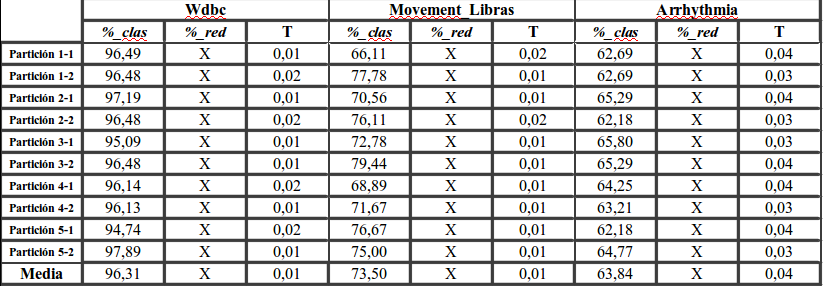
\includegraphics[width=1.0\linewidth]{3NN}
\caption{Tabla de resultados para 3NN}
\label{fig:3NN}
\end{figure}


\begin{figure} [H]
\centering
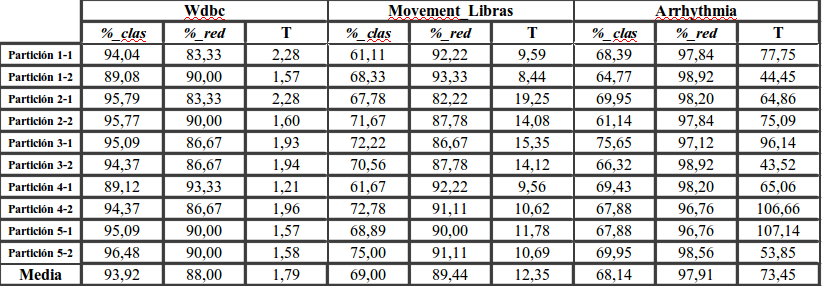
\includegraphics[width=1.0\linewidth]{SFS}
\caption{Tabla de resultados para SFS}
\label{fig:SFS}
\end{figure}


\begin{figure} [H]
\centering
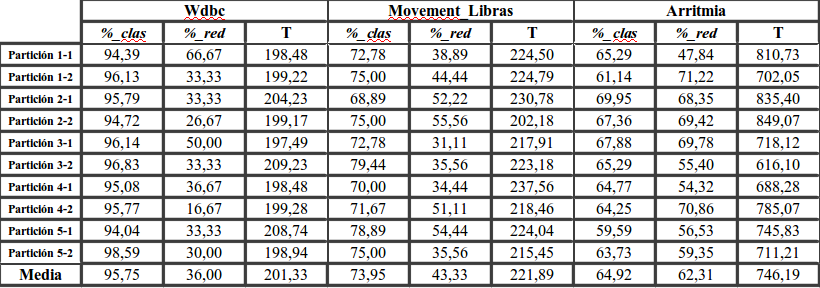
\includegraphics[width=1.0\linewidth]{AM1}
\caption{Tabla de resultados para el primer algoritmo memético}
\label{fig:AM1}
\end{figure}


\begin{figure} [H]
\centering
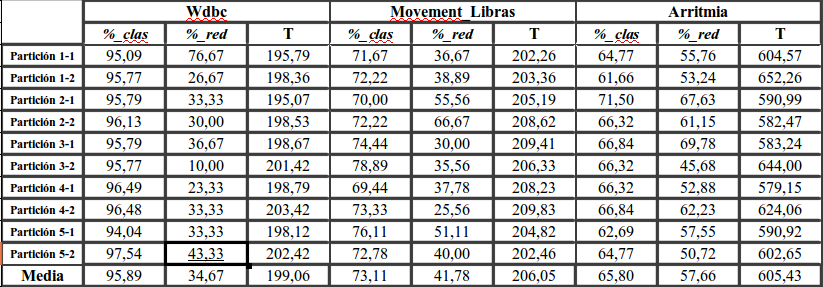
\includegraphics[width=1.0\linewidth]{AM2}
\caption{Tabla de resultados para el segundo algoritmo memético}
\label{fig:AM2}
\end{figure}

\begin{figure} [H]
\centering
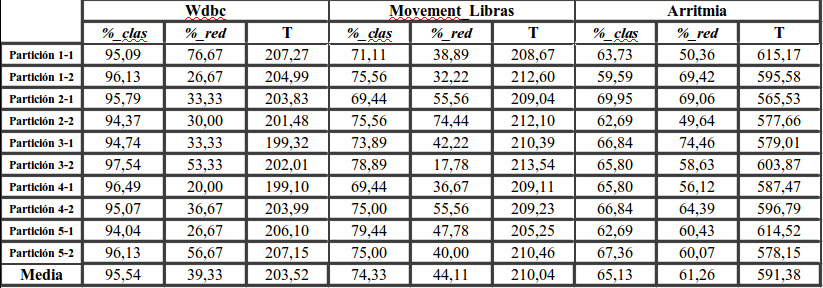
\includegraphics[width=1.0\linewidth]{AM3}
\caption{Tabla de resultados para el tercer algoritmo memético}
\label{fig:AM3}
\end{figure}


\begin{figure} [H]
\centering
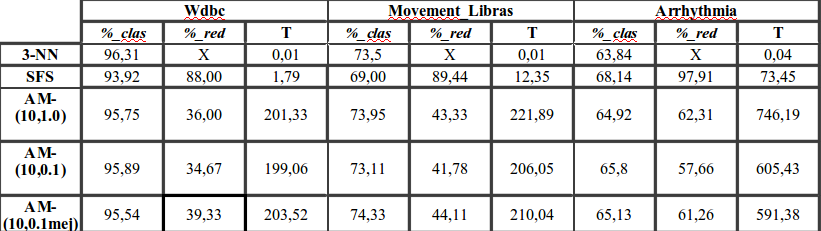
\includegraphics[width=1.0\linewidth]{todos}
\caption{Tabla global de resultados}
\label{fig:todos}
\end{figure}

Como podemos observar, en la primera base de datos (WDBC) los algoritmos implementados no superan la tasa de clasificación de 3NN. Como ya he comentado en prácticas anteriores, WDBC tiene muy poco ruido y es muy posible que todas sus características o la mayoría de ellas sean importantes. Esto justifica que cuanto más tasa de reducción haya, peor tasa de clasificación. El mejor resultado nos lo da el segundo algoritmo memético, el cual tiene la menor tasa de reducción.
\\
\\
En cuanto a la segunda base de datos, los tres algoritmos superan en tasa de clasificación a SFS y solo superan a 3NN el primer memético y el tercero. El hecho de que el primer algoritmo y el tercero obtengan mejores resultados que el segundo podría deberse a que el segundo puede realizar la explotación sobre soluciones no tan buenas. El primero realiza la explotación sobre todas las soluciones (incluyendo las mejores) y el tercero sobre las mejores.
\\
\\
En la tercera base de datos vemos una contradicción respecto a lo explicado en el anterior párrafo, ya que ahora el segundo algoritmo es mejor que los demás (aunque no superan a SFS). La posible explicación que le veo es que al realizar búsqueda local sobre soluciones que no son necesariamente las mejores, crea más diversidad, es decir, explota soluciones posiblemente peores y evita caer en los óptimos locales de las mejores. Podría tener sentido esta explicación ya que el campo de búsqueda de la base de datos de arrhythmia es muy grande. Al ser tan ruidosa esta base de datos, SFS obtiene mejores resultados (con bastante diferencia) que los demás algoritmos. SFS empieza explorando una solución vacía, por lo que su tasa de reducción es muy alta y al ser tan ruidosa la BD esto le da más calidad.

\end{document}